\documentclass[12pt,a4paper]{article}
\usepackage[polish]{babel}
\usepackage{graphicx}
\usepackage[margin=2cm]{geometry}
\usepackage[T1]{fontenc}
\usepackage{hyperref}
\usepackage{url}
\usepackage[]{algorithm2e}
\usepackage{listings}
\usepackage{algorithm}
\usepackage[noend]{algpseudocode}
\usepackage{tikz}
\usetikzlibrary{positioning}
\usepackage[utf8]{inputenc}
\usepackage{lmodern}

\selectlanguage{polish}


\begin{document}
\clearpage

\begin{figure}[h]
\centering

\includegraphics[width=0.25\textwidth]{images/ps-logo.png}
\end{figure}

\begin{center}
\large{Wydział Matematyki Stosowanej}
\end{center}
\begin{center}
\large{Kierunek Informatyka}
\end{center}
\begin{center}
\large{Studia stacjonarne I stopnia}
\end{center}

\hspace{6cm}

\begin{center}
\Huge\textbf{Projekt Inżynierski}
\end{center}
\begin{center}
\Large{Gra sieciowa w środowisku aplikacji webowej - Szachy}
\end{center}

\hspace{6cm}
\\\\


\begin{minipage}[t]{0.45\textwidth}
\begin{center}
\normalsize{\textbf{Kierujący projektem:}\\dr inż. Zdzisław Sroczyński}
\end{center}
\end{minipage}
\hfill
\begin{minipage}[t]{0.45\textwidth}
\begin{center}
\normalsize{\textbf{Autor:}\\Bruno Masłoń}
\end{center}
\end{minipage}

\vfill

\begin{center}
Gliwice, 2025
\end{center}

\newpage

\pagenumbering{arabic}
\tableofcontents

\newpage
\section{Wstęp}
\subsection{Opis projektu - streszczenie}
    

Projekt BRNChess to aplikacja webowa, składająca się z dwóch głównych elementów - aplikacji internetowej (frontend), stworzonej w oparciu o technologie React + Vite, pisana w języku typescript oraz aplikacji serwerowej (backend), zbudowanej na platformie .NET Framework. 
\\

Aplikacja ta ma na celu umożliwienie użytkownikom rozgrywkę w jedną z najpopularniejszych gier pvp na świecie, jaką są szachy. Szachy to gra planszowa dla dwóch graczy, z których każdy kontroluje zestaw figur szachowych, a celem jest zaszachowanie króla przeciwnika, tj. zagrożenie mu nieuchronnym schwytaniem. Zasady gry w szachy, które są znane dzisiaj, pojawiły się w Europie pod koniec XV wieku, a ich standaryzacja i powszechna akceptacja nastąpiła pod koniec XIX wieku. Aplikacja umożliwia na rozegranie partii online wraz z innymi użytkownikami z całego świata jak na rozegranie meczu przeciwko silnikowi szachowemu. Dzięki dotnetowej paczce SignalR gra może toczyć się w czasie rzeczywistym przez co możliwe jest wykorzystanie kontroli czasowej podczas przebiegu partii, co wspiera częstsze odwiedziny strony internetowej.

\subsection{Główne założenia i cele projektu}

\begin{itemize}
\item \textbf{Gra online:} Stworzenie aplikacji do gry w szachy online, jest głównym założeniem projektu. Gracze zostają dobierani w sposób losowy, w oparciu o ich obecną punktację.
\item \textbf{Gra offline:} Integracja z opensourceowym projektem silnika szachowego "Stockfish", w celu umożliwienia użytkownikom gry z komputerem.
\item \textbf{Gra ze znajomymi} Utworzenie systemu relacji pomiędzy użytkownikami, aby użytkowcy mogli rozgrywać partie ze swoimi znajomymi oraz w celu umożliwiania tworzenia własnych gier, niebędących przypadkowym wyborem.
\item \textbf{Interfejs} Bardzo ważnym elementem współczesnych aplikacji jest interfejs użytkownika. Cały UI powinien być intuicyjny oraz przyjemny dla oka. Dobrane odpowiedniej stylistyki strony jak i jej poszczególnych elementów jest kluczowe, aby użytkowcy chętnie wybierali odwiedzali platforme.
\item \textbf{Konto użytkownika} Zaprojektowanie kąt użytkowników, na których przechowywane będą wszystkie i dane, aktywności jak i osiągnięcia zdobywane podczas użytkowania aplikacji.
\item \textbf{Bezpieczeństwo danych} Dane przekazywane przez użytkowników, powinny być przechowywane w sposób bezpieczny, w szczelności dane wrażliwe.
\item \textbf{Hosting}
\item \textbf{Dodatkowe funkcjonalności} Do dodatkowych funkcjonalności można zaliczyć między innymi: globalny ranking graczy jak i wśród znajomych, przegląd gier użytkownika, czy personalizacje konta i ustawień gry.
    
\end{itemize}

\newpage
\section{Stos technologiczny}
\subsection{Aplikacja internetowa - frontend}
\subsubsection{Javascript}
JavaScript jest używany najczęściej przy tworzeniu stron www, zapewniając ich interaktywność oraz obsługę zdarzeń, walidację formularzy czy budowanie elementów nawigacyjnych. Ale w tym języku można także pisać pełnoprawne aplikacje (korzystając z frameworków do budowania aplikacji jak np. Angular, React czy Vue – o nich za chwilę). Javascript może też być wykorzystywany do tworzenia gier w przeglądarkach, a jednym z popularnych frameworków do tego celu jest Phaser. JS-a można używać również po stronie serwera (backend) dzięki frameworkowi Node.

\subsubsection{Typescript}
TypeScript to język programowania stworzony przez Microsoft w 2012 roku. Jego twórcą jest Anders Hejlsberg, znany również jako ojciec języka C\#. TypeScript jest nadzbiorem JavaScriptu, co oznacza, że każdy poprawny kod JS jest równocześnie poprawnym kodem TS. W praktyce TypeScript rozszerza możliwości JavaScriptu o opcjonalne statyczne typowanie, nowe struktury danych, takie jak Enumy i Klasy, oraz inne funkcje wymienione w dalszej części artykułu. TS posiada też aktywną społeczność programistów tworzących biblioteki, które ułatwiają pracę programistom poprzez dodawanie typowania do już istniejących projektów JS. Dzięki temu są one przystosowane do pracy z TypeScriptem.
\\\\
Głównym celem powstania TypeScriptu było wprowadzenie silniejszego systemu typów do JavaScriptu, które pozwalają na odgórne ustalanie rodzajów zdefiniowanych przez dewelopera zmiennych, aby ułatwić tworzenie dużych, skalowalnych aplikacji. Język ten stał się popularny wśród deweloperów dzięki swojej elastyczności, możliwościom oferowanym przez statyczne typowanie oraz łatwości integracji z istniejącymi projektami JS.
\\\\
TypeScript różni się od JavaScriptu głównie wspomnianym systemem typów, który pozwala na lepsze zarządzanie i kontrolowanie kodu. Dodatkowo TypeScript wprowadza takie elementy jak interfejsy, klasy abstrakcyjne czy dekoratory, co sprawia, że kod staje się bardziej przejrzysty i łatwiejszy w utrzymaniu.

\subsubsection{React}
React to biblioteka JavaScript służąca do renderowania interfejsów użytkownika (UI). Interfejs użytkownika składa się z małych jednostek, takich jak przyciski, tekst i obrazy. React pozwala łączyć je w komponenty wielokrotnego użytku, które można zagnieżdżać. Od stron internetowych po aplikacje na telefony, wszystko na ekranie można podzielić na komponenty. Każdy komponent Reacta jest funkcją JavaScript, która może zawierać pewne znaczniki renderowane przez Reacta w przeglądarce. Komponenty Reacta używają rozszerzenia składni o nazwie JSX do reprezentowania tych znaczników. JSX wygląda bardzo podobnie do HTML, ale jest nieco bardziej rygorystyczny i może wyświetlać dynamiczne informacje. 

\subsubsection{Vite}
Vite to narzędzie do budowania, które ma na celu zapewnienie szybszego i bardziej oszczędnego doświadczenia programistycznego dla nowoczesnych projektów internetowych.
\\\\
Vite.js to nowoczesne i wydajne środowisko do budowania aplikacji front-end, stworzone przez twórcę Vue.js - Evana You. Jest on znany ze swojej niewiarygodnej szybkości, dzięki wykorzystaniu natywnych modułów ES dla przyspieszonego hot module replacement (HMR) oraz kompilacji w przeglądarce. Vite.js przełamuje tradycyjne bariery w budowie aplikacji, eliminując konieczność korzystania z bundlerów takich jak Webpack czy Rollup. Jego modularna architektura oraz wsparcie dla wielu ramkowych, w tym Vue, React czy Preact, czynią go uniwersalnym i elastycznym narzędziem dla dowolnego developera front-end.

\subsubsection{Sass / SCSS}
Sass to preprocessor CSS, który umożliwia programowanie styli w znacznie bardziej efektywny i zorganizowany sposób niż zwykły CSS. Pozwala na definiowanie stałych, zagnieżdżanie reguł CSS, używanie zmiennych, funkcji, operatorów i wiele więcej. Dzięki temu, można wykorzystać Sass do szybszego i łatwiejszego tworzenia stylów strony, a także czytać i zarządzać istniejącym kodem znacznie lepiej. Jest to szczególnie przydatne w przypadku dużych projektów, gdzie style są rozbudowane i trudne do zarządzania.

\subsection{Aplikacja serwerowa - backend}
\subsubsection{C\#}
C\# jest nowoczesnym, obiektowym językiem wysokiego poziomu, który został opracowany na zlecenie Microsoft już w latach 1998 - 2001. Pod względem składni porównuje się go często do języków takich, jak Object Pascal, C++ i Java. W środowisku programistycznym uznawany jest za prosty, przyjazny i przejrzysty. C\# jest ściśle związany z platformą .NET, która stanowi dla niego framework i środowisko uruchomieniowe zarazem. Przez długi czas ta zależność wskazywana była jako największa wada języka, bowiem ograniczała jego zastosowanie jedynie do systemów Windows. Microsoft rozprawił się z tym problemem w 2016 roku, publikując .NET Core - kompatybilny również z innymi systemami operacyjnymi. Od tego czasu C\# służy do budowy programów i aplikacji na wszystkie systemy operacyjne.

\subsubsection{.NET Framework}
.NET Framework to środowisko wykonywania w czasie wykonywania, które zarządza aplikacjami docelowymi .NET Framework. Składa się ze środowiska uruchomieniowego języka wspólnego, które zapewnia zarządzanie pamięcią i inne usługi systemowe, oraz rozbudowanej biblioteki klas, która umożliwia programistom korzystanie z niezawodnego kodu dla wszystkich głównych obszarów opracowywania aplikacji.

\subsubsection{PostgreSQL}
PostgreSQL to system lub silnik baz danych kompatybilny z usługami OVHcloud i większością popularnych narzędzi. Obsługuje różne modele danych w celu tworzenia wydajnych i skalowalnych aplikacji zorientowanych obiektowo. Umożliwia pracę ze złożonymi zbiorami danych, bez spowolnień. Ułatwia przechowywanie, odczyt i zapis danych. Oferujemy możliwość korzystania z PostgreSQL za pośrednictwem usług cloud i naszych rozwiązań hostingowych.



\subsection{Narzędzia pomocnicze}

\subsubsection{GIT}
Git to rozproszony system kontroli wersji, co oznacza, że lokalny klon projektu jest kompletnym repozytorium kontroli wersji. Te w pełni funkcjonalne repozytoria lokalne ułatwiają pracę w trybie offline lub zdalnie. Deweloperzy zatwierdzają swoją pracę lokalnie, a następnie synchronizują kopię repozytorium z kopią na serwerze. Ten paradygmat różni się od scentralizowanej kontroli wersji, w której klienci muszą synchronizować kod z serwerem przed utworzeniem nowych wersji kodu.
\\\\
Elastyczność i popularność usługi Git sprawiają, że jest to doskonały wybór dla dowolnego zespołu. Wielu deweloperów i absolwentów uczelni już wie, jak korzystać z usługi Git. Społeczność użytkowników usługi Git utworzyła zasoby do szkolenia deweloperów i popularności usługi Git, aby ułatwić uzyskanie pomocy w razie potrzeby. Prawie każde środowisko programistyczne ma obsługę usługi Git i narzędzia wiersza polecenia Git zaimplementowane w każdym głównym systemie operacyjnym.

\subsubsection{Github}
GitHub jest serwisem, który służy do współpracy przy tworzeniu kodu. Jest jednym z najpopularniejszych serwisów internetowych hostujących repozytoria Git w chmurze. Obsługiwane obszary serwisu obejmują nie tylko przechowywanie kodu, ale również zbieranie informacji o błędach, zarządzanie projektem oraz wszystkie niezbędne procesy automatycznego budowania i testowania aplikacji. Właśnie dlatego GitHub stał się centrum skupiającym programistów i środowisko otwartego oprogramowania.
\\\\
Serwisy typu GitHub stanowią stopień pośredni pomiędzy wykorzystaniem serwisu Git w tradycyjny sposób a systemami scentralizowanymi.

\subsubsection{Sourcetree}
Sourcetree to graficzny klient umożliwiający dostęp do repozytoriów Git i Mercurial z systemów Windows oraz MacOS, który pomaga wizualizować rozwój bez konieczności korzystania z wiersza polecenia.

\subsubsection{Postman}
Postman to narzędzie, które ułatwi nam pracę z API poprzez przejrzysty graficzny interfejs. Oferuje wiele funkcjonalności, dzięki którym poza prostym wywołaniem endpointu, który jest pojedynczym adresem odpowiedzialnym za daną usługę, jesteśmy w stanie zrobić o wiele więcej, o czym wspomnimy w dalszej części tego artykułu. Postman jest używany przez ponad 500 tysięcy firm na całym świecie, a dzięki swojej popularności, oferuje stałe wsparcie i rozwija swoje usługi.
\\\\
Podstawowy plan korzystania z tego narzędzia jest bezpłatny, a w jego ramach dostępne są wszystkie podstawowe funkcjonalności. Kolejne plany oparte są na miesięcznej subskrypcji i dają możliwość pracy przy bardziej zaawansowanych projektach, do których zaangażowana jest większa liczba osób.

\subsubsection{Figma}
Figma to jedno z nowocześniejszych i cieszących się dużą popularnością narzędzi do projektowania i prototypownia stron internetowych i aplikacji mobilnych. Umożliwia tworzenie interaktywnych widoków w przeciwieństwie do statycznych makiet. Posiada bardzo uproszczony interfejs, a przy tym jest bardzo funkcjonalne. Figma zawiera jedynie niezbędne pakiety i narzędzia najczęściej wykorzystywane w pracy Web Designera, co przedkłada się na stosunkową małą wagę całego programu. Jego podstawową zaletą jest szybkość działania mimo otwartych kilkunastu widoków jednocześnie. Dodatkowo za pomocą Figmy można łatwo edytować dowolne pliki wektorowe w tym SVG, co znacznie przyspiesza pracę nad projektem.

Figma jako zewnętrzny program zalazła zastosowanie w projekcie głownie do projektowania własnych ikon, nieistniejących bądź niedostępnych bezpłatnie na internecie. Zastosowanie prostego, ale bardzo efektywnego narzędzia ma duże znaczenie dla rozwoju aplikacji gry mobilnej, w szczegolnosci nakierowanej na przyjemny dla uzytkownika interface. Dodatkowo Figma posłużyła do zaprojektowania i utworzenie modeli bierek do gry w szachy.  

\newpage



\section{Opis implementacji}
    \subsection{System kontroli wersji}

W tym projekcie kontrola wersji jest zarządzana za pomocą Git i GitHub, z Sourcetree jako aplikacją desktopową do interakcji. Taka konfiguracja zapewnia zorganizowany i wydajny przepływ pracy w zakresie śledzenia zmian, współpracy i utrzymywania integralności bazy kodu.

\newpage

    \subsection{Warstwa danych}
        \subsubsection{Schemat bazy danych}

\textbf{Relacje użytkownika}\\
Segment relacji z użytkownikami obejmuje kilka encji i ich relacji, które zarządzają danymi użytkownika. Encja User jest rdzeniem tego segmentu i jest powiązany z wieloma innymi jednostkami. Każdy użytkownik jest powiązany z rolą, która definiuje uprawnienia użytkownika w systemie, a relacja między nimi jest ustanawiana za pomocą klucza obcego na RoleId. Ponadto każdy użytkownik jest powiązany z kodem weryfikacyjnym do celów weryfikacji, a relacja ta jest jeden do jednego. Encje UserProfileImage i UserBackgroundImage przechowują dane związane z obrazem, tworząc relacje jeden-do-jednego z podmiotem User. Jednostki UserElo i UserStats śledzą odpowiednio ranking i statystyki użytkownika i są również powiązane z jednostką User poprzez relacje jeden-do-jednego.

\begin{figure}[h!]
    \centering
    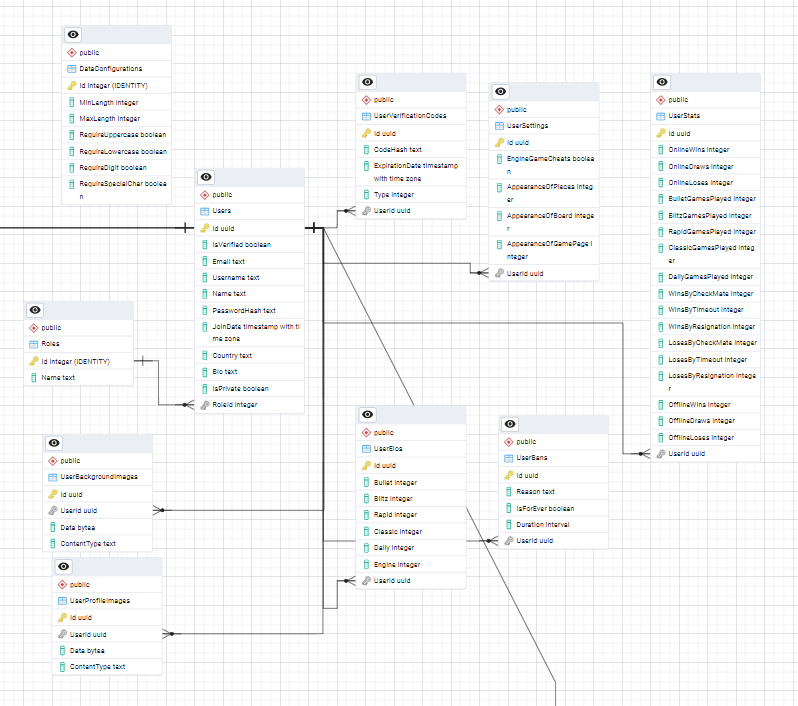
\includegraphics[width=0.8\textwidth]{zdj/user_ERD.png}
    \caption{Diagram relacji jednostka-relacja przedstawiający relacje użytkownika.}
    
\end{figure}
\newpage

\textbf{Relacje znajomości}\\
Segment relacji przyjaźni jest zarządzany przez jednostkę przyjaźni, która reprezentuje połączenia społeczne między użytkownikami. Każda Encja Friendship ma dwóch kluczowych uczestników: Requestor (przyjmujacy) i Receiver (odbierający). Są to obaj użytkownicy, a relacje między tymi podmiotami są modelowane za pomocą kluczy obcych: RequestorId i ReceiverId. Ta relacja jest wiele-do-jednego, co oznacza, że użytkownik może mieć wiele przyjaźni zarówno jako żądający, jak i odbiorca. Dodatkowo, jednostka FriendshipStats śledzi statystyki związane z każdą przyjaźnią, tworząc relację jeden-do-jednego z jednostką Friendship.

\begin{figure}[h!]
    \centering
    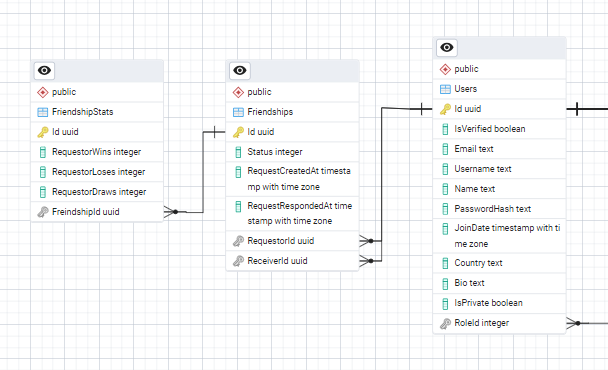
\includegraphics[width=0.8\textwidth]{zdj/friendship_ERD.png}
    \caption{Diagram relacji między podmiotami przedstawiający relacje przyjaźni między użytkownikami.}
    
\end{figure}
\newpage

\textbf{Relacje w grach sieciowych}\\
Segment Web Game Relations obsługuje strukturę internetowej gry w szachy, z kilkoma jednostkami, które śledzą różne aspekty gry. Jednostka WebGame reprezentuje samą grę, łącząc graczy (WhitePlayer i BlackPlayer) poprzez relacje jeden-do-jednego. Stan i czas gry są kontrolowane przez encje WebGameState i WebGameTiming, które są połączone za pomocą kluczy obcych. Jednostka WebGamePlayer służy do śledzenia informacji specyficznych dla gracza dla każdej gry i odwołuje się do jednostki User. Ruchy wykonane w grze są przechowywane w encji WebGameMove, która ma relację wiele do jednego z WebGame. Dodatkowo, wiadomości wymieniane podczas gry są obsługiwane przez encje WebGameMessage i WebGamePlayerMessage, tworzące relacje odpowiednio z WebGame i WebGamePlayer.

\begin{figure}[h!]
    \centering
    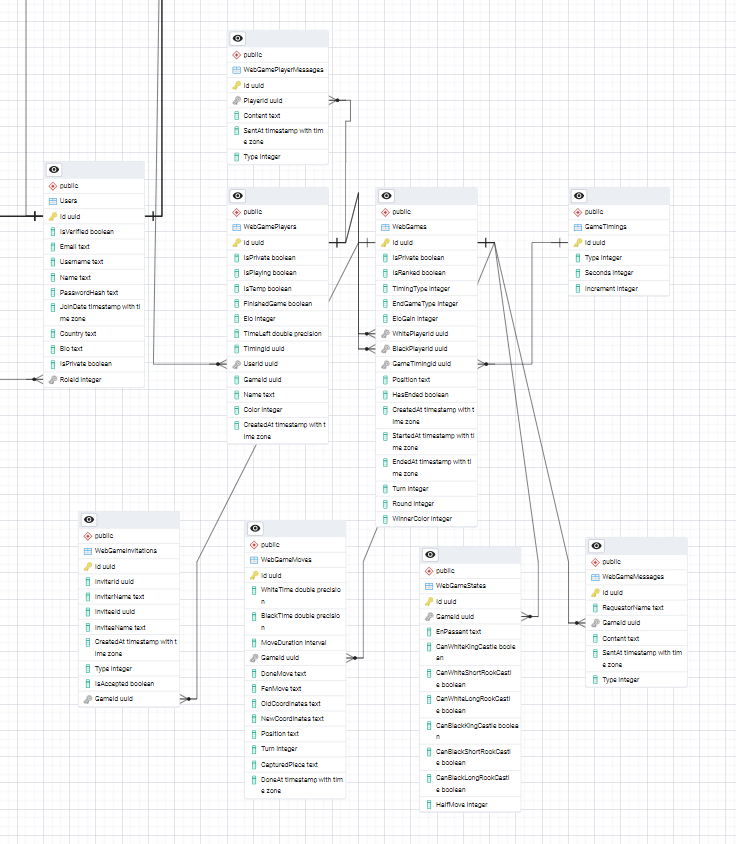
\includegraphics[width=0.8\textwidth]{zdj/online_ERD.png}
    \caption{Diagram relacji między podmiotami ilustrujący strukturę interakcji w grach sieciowych.}
    
\end{figure}
\newpage

\textbf{Relacje w grach z silnikiem}\\
Segment ten skupia się na aspekcie gry opartym na silniku, gdzie każda gra jest zarządzana przez encję EngineGame. Encja EngineGame jest powiązana z encją EngineGamePlayer, reprezentującą użytkownika, który gra w grę opartą na silniku, a relacja jeden-do-jednego jest ustanawiana poprzez PlayerId. Każdy ruch w grze jest przechwytywany w encji EngineGameMove, która jest powiązana z encją EngineGame poprzez klucz obcy. Encja EngineGameState przechowuje aktualny stan gry opartej na silniku i jest powiązana z EngineGame poprzez relację jeden-do-jednego. Dodatkowo, wiadomości specyficzne dla gier silnikowych są przechowywane w encji EngineGameMessage, która jest powiązana z EngineGame poprzez klucz obcy.

\begin{figure}[h!]
    \centering
    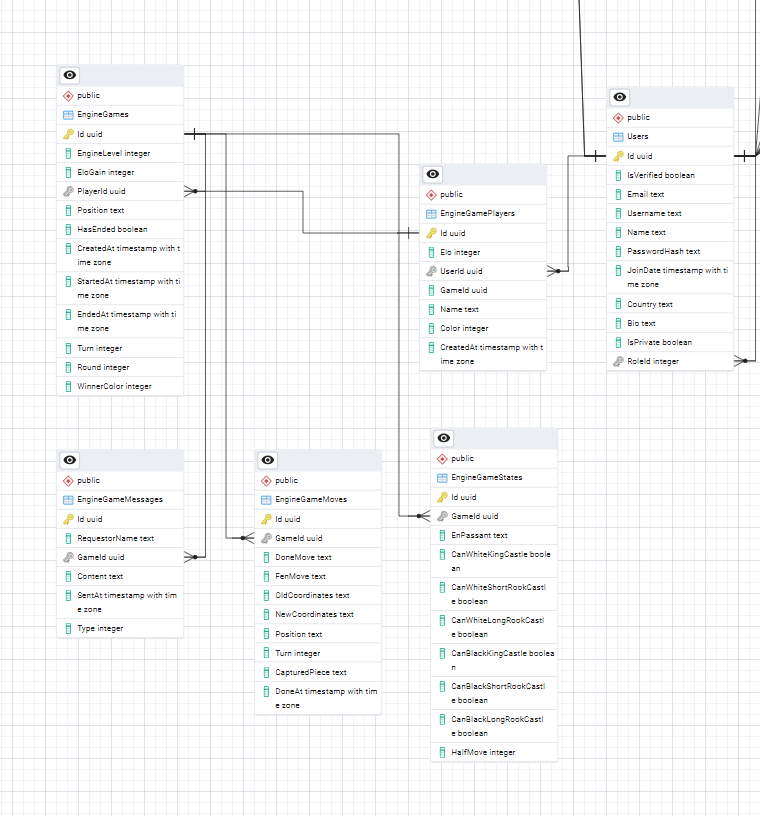
\includegraphics[width=0.8\textwidth]{zdj/offline_ERD.png}
    \caption{Diagram zależności między jednostkami przedstawiający relacje między silnikiem a grą.}
    
\end{figure}
\newpage


        \subsubsection{Opis encji}
\begin{itemize}
    \item \textbf{DataConfigurations} -Zawiera ustawienia konfiguracji dla kluczowych pól użytkownika. Brak relacji. Służy jako tablica konfiguracyjna z danymi wstępnymi (np. długość hasła).
    \item \textbf{Roles} - Określa role użytkowników w systemie, takie jak "User" i "Admin". Jedna rola może być przypisana wielu użytkownikom.
    \item \textbf{Users} - Główna encja reprezentująca użytkownika.
    \begin{itemize}
        \item Każdy użytkownik ma przypisaną jedną rolę.
        \item Użytkownik posiada jedno zdjęcie profilowe oraz tło profilu.
        \item Jeden użytkownik ma przydzieloną tablicę statystyk oraz ustawień.
        \item Każdy użytkownik posiada jedną tablicę Elo zawierającą punktację gracza.
        \item Jeden użytkownik może mieć przypisy jeden kod weryfikacyjny konta.
        \item Użytkownik może być w wielu relacja z innymi użytkownikami odwzorowanymi w tabli Friendships.
        \item Użytkownik posiada listę graczy, rozdzieloną na dwie tablice w zależności czy gracz dotyczy gry online czy offline. Użytkownik może być przypisany do wielu gry online jak i offline.
    \end{itemize}
    \item \textbf{UserProfileImage} - zdjęcia profilowe użytkownika. Każde zdjęcie należy do jednego użytkownika.
    \item \textbf{UserBackgroundImages} - tło profilu użytkownika. Każde tło należy do jednego użytkownika.
    \item \textbf{UserElos} - punktacja użytkownika dla poszczególnych trybów czasowych gry. Jeden użytkownik ma przypisaną jedną punktację.
    \item \textbf{UserStats} - tablica statystyki użytkownika. Jedne statystyki są przypisane do jednego użytkownika.
    \item \textbf{UserSettings} - globalne ustawienia konta oraz gier. Jedne ustawienia są przypisane do jednego użytkownika.
    \item \textbf{UserVerificationCodes} - tablica kodów weryfikacyjnych. Jeden kod weryfikacyjny należy do jednego użytkownika.
    \item \textbf{Friendships} - tablica relacji pomiędzy użytkownikami.
    \begin{itemize}
        \item Tablica ta posiada dwa pola referencji do użytkownika - Requestor i Receiver, w zależności od tego, kto zazadał (czyli utworzył) relacji.
        \item Każda relacja posiada jedną tablicę statyk.
    \end{itemize}
    \item \textbf{FriendshipStats} - Statystki dotyczące relacji uzytkownikow.
    \item \textbf{WebGames} - Gry online między użytkownikami.
    \begin{itemize}
        \item Każda gra ma przypisaną jedną konfigurację czasową.
        \item Gra posiada odwołanie do jednego stanu gry, oraz listy powstałych ruchów i  wiadomości.
        \item Do każdej gry przypisanych jest dwóch graczy online, nazwanych odpowiednio: biały i czarny, w zależności do koloru bierek gracza.
    \end{itemize}
    \item \textbf{GameTimings} - kontrole czasowe dla gier z ograniczeniem czasu. Jeden zestaw czasowy może być używany w wielu grach.
    \item \textbf{WebGameStats} - Stan gry online, przechowuje dane szczególne dotyczące obecnej gry. Jeden stan jest przypisany do jednej gry.
    \item \textbf{WebGameInvitations} - Opcjonalne zaproszenia do gry. Jedno zaproszenie przypisane jest do jeden gry i istnieje tylko w przypadku prywatnych gier.
    \item \textbf{WebGameMessages} - Wiadomości systemowe dotyczące gry online. Wiele wiadomości może być przypisanych do jednej gry.
    \item \textbf{WebGameMove} - Ruchy wykonane podczas gry online. Wiele ruchów może należeć do jednej gry.
    \item \textbf{WebGamePlayers} - Tablica graczy gry online. Gracz może być przypisany tylko do jeden gry jak biały lub czarny.
    \item \textbf{WebGamePlayerMessages} - wiadomości wysłane przez graczy podczas gry online.
    \item \textbf{EngineGames} - Tablica gier offline z silnikiem szachowym. Posiada jednego gracza, którym jest użytkownik.
    \item \textbf{EngineGameStats} - Stan gry offline, przechowuje dane szczególne dotyczące obecnej gry. Jeden stan jest przypisany do jednej gry.
    \item \textbf{EngineGamePlayers} - Gracze gier offline. Gracz może być przypisany tylko do jeden gry jak biały lub czarny.
    \item \textbf{EngineGameMoves} - Ruchy wykonane podczas gry offline. Wiele ruchów należy do jednej gry.
    \item \textbf{EngineGameMessages} - Automatyczne wiadomości dotyczące gry offline. Wiele wiadomości należy do jednej gry.
\end{itemize}


    \subsection{Backend}
        \subsubsection{Architektura}



        \subsubsection{Wykorzystane pakiety i biblioteki}

W projekcie zastosowano szereg bibliotek, które wspierają rozwój i funkcjonalność aplikacji. Każda z wymienionych bibliotek została dobrana w celu spełnienia konkretnych wymagań funkcjonalnych i architektonicznych projektu, co pozwala na jego rozwój zgodny z najlepszymi praktykami. Poniżej przedstawiono szczegółowy opis wybranych komponentów:
\begin{itemize}
    \item \textbf{SignalRSwaggerGen}: SignalRSwaggerGen umożliwia integrację SignalR z generatorem dokumentacji Swagger. Dzięki temu można dokumentować huby SignalR w podobny sposób, jak w przypadku typowych API REST. To znacznie upraszcza korzystanie z SignalR w projektach, gdzie przejrzystość i zrozumiałość API jest kluczowa.
    \item \textbf{Swashbuckle.AspNetCore}: Swashbuckle to jedno z najpopularniejszych narzędzi do generowania dokumentacji Swagger w projektach ASP.NET Core. Umożliwia automatyczne generowanie interaktywnej dokumentacji API, która może być używana do testowania endpointów bezpośrednio z poziomu przeglądarki.
    \item \textbf{AutoMapper}: AutoMapper jest biblioteką ułatwiającą mapowanie obiektów, co pozwala na szybkie i bezbłędne przekształcanie danych pomiędzy różnymi warstwami aplikacji, np. z warstwy domenowej na DTO (Data Transfer Object) i odwrotnie. Dzięki temu eliminuje potrzebę ręcznego mapowania, co zmniejsza ryzyko błędów i przyspiesza rozwój.
    \item \textbf{MediatR}: MediatR implementuje wzorzec Mediatora, umożliwiając luźne powiązania pomiędzy komponentami aplikacji. Jest szeroko stosowany w aplikacjach opartych na wzorcu CQRS (Command Query Responsibility Segregation). Dzięki MediatR można łatwo zarządzać logiką obsługi zdarzeń i zapytań, co poprawia modularność i testowalność kodu.
    \item \textbf{Npgsql.EntityFrameworkCore.PostgreSQL}: Jest to dostawca Entity Framework Core dla bazy danych PostgreSQL. Umożliwia korzystanie z zaawansowanych funkcji PostgreSQL, takich jak typy JSON, tablice czy rozszerzenia specyficzne dla tej bazy danych, bezpośrednio w ramach Entity Framework Core.
    \item \textbf{FluentAssertions}: FluentAssertions to biblioteka, która rozszerza możliwości standardowych asercji w testach jednostkowych. Umożliwia pisanie bardziej czytelnych i wyrażających zamiar asercji, takich jak result.Should().Be(expected) zamiast standardowego Assert.AreEqual(expected, result). Jest szeroko wykorzystywana w testach jednostkowych, ponieważ zapewnia lepszą czytelność i kontrolę nad wynikami testów.

    \item \textbf{Microsoft.AspNetCore.SignalR}: To biblioteka w ekosystemie .NET, która umożliwia łatwe dodanie funkcjonalności komunikacji w czasie rzeczywistym do aplikacji webowych. SignalR abstrahuje nad złożonością protokołów komunikacji (takich jak WebSockets, Long Polling) i pozwala na łatwą wymianę danych w czasie rzeczywistym między serwerem a klientami, bez konieczności odświeżania strony. SignalR jest szczególnie użyteczny w aplikacjach wymagających bieżącej interakcji z użytkownikiem, takich jak czaty, powiadomienia, gry online, a także aplikacje, które wymagają synchronizacji danych w czasie rzeczywistym (np. aplikacje finansowe, analityczne).
    \item \textbf{Microsoft.AspNetCore.OpenApi}: Biblioteka ta umożliwia integrację z OpenAPI, co pozwala na automatyczne generowanie dokumentacji API. Jest to szczególnie użyteczne w przypadku projektów opartych na architekturze REST, ponieważ pozwala deweloperom i użytkownikom końcowym lepiej rozumieć działanie aplikacji oraz dostępne endpointy.
    \item \textbf{Microsoft.AspNetCore.Cors}: Biblioteka ta obsługuje Cross-Origin Resource Sharing (CORS), co umożliwia kontrolowanie, które domeny mają dostęp do zasobów serwera. Jest to kluczowe w aplikacjach internetowych komunikujących się z frontendem hostowanym na innych domenach.
    \item \textbf{Microsoft.AspNetCore.Identity}: Microsoft.AspNetCore.Identity dostarcza rozbudowany framework do zarządzania użytkownikami, rolami, uwierzytelnianiem i autoryzacją. Umożliwia łatwą integrację takich funkcji, jak rejestracja, logowanie, resetowanie haseł czy zarządzanie rolami użytkowników.
    \item \textbf{Microsoft.AspNetCore.Http.Abstractions}: Biblioteka dostarcza podstawowe interfejsy i klasy wspierające obsługę żądań i odpowiedzi HTTP w aplikacjach ASP.NET Core. Umożliwia budowanie lekkich middleware oraz operacje na poziomie HTTP, takie jak praca z HttpContext.
    \item \textbf{Microsoft.AspNetCore.Authentication.JwtBearer}: Biblioteka ta obsługuje uwierzytelnianie oparte na JWT (JSON Web Tokens) w aplikacjach ASP.NET Core. Jest często używana w nowoczesnych aplikacjach webowych i API do implementacji bezpiecznych mechanizmów uwierzytelniania i autoryzacji.
    \item \textbf{Microsoft.AspNetCore.Mvc.Core}: Biblioteka ta zawiera podstawowe funkcje MVC (Model-View-Controller) dla aplikacji ASP.NET Core. Jest wykorzystywana do budowy endpointów API oraz obsługi żądań HTTP, zapewniając spójność i elastyczność w projektowaniu warstwy prezentacji i komunikacji.
    \item \textbf{Microsoft.AspNetCore.Mvc.Testing}: Biblioteka ta umożliwia łatwe testowanie aplikacji ASP.NET Core z wykorzystaniem WebApplicationFactory, które pozwala na uruchomienie aplikacji w testowym środowisku. Jest to kluczowa biblioteka do testów integracyjnych, ponieważ pozwala na testowanie całej aplikacji lub jej części, w tym kontrolerów, routingu i middleware, bez potrzeby uruchamiania pełnego serwera.
    \item \textbf{Microsoft.IdentityModel.Tokens}: Jest to kluczowa biblioteka do obsługi tokenów, takich jak JWT (JSON Web Tokens). Umożliwia tworzenie i weryfikację tokenów, co jest niezbędne w aplikacjach z uwierzytelnianiem i autoryzacją opartą na tokenach.
    \item \textbf{Microsoft.EntityFrameworkCore}: Entity Framework Core to nowoczesny ORM (Object-Relational Mapper) dla platformy .NET. Umożliwia łatwe mapowanie obiektów w aplikacji na tabele w relacyjnej bazie danych. Zapewnia wsparcie dla wielu funkcji, takich jak zapytania LINQ, migracje schematów bazy danych czy śledzenie zmian w danych.
    \item \textbf{Microsoft.EntityFrameworkCore.Tools}: Narzędzie wspomagające pracę z Entity Framework Core. Umożliwia m.in. zarządzanie migracjami, tworzenie baz danych na podstawie modelu aplikacji oraz generowanie kodu odwrotnego (reverse engineering) z istniejącej bazy danych. Ustawienie PrivateAssets na all powoduje, że biblioteka ta nie jest uwzględniana w pakiecie wynikowym, ponieważ jej funkcje są wykorzystywane głównie podczas rozwoju aplikacji.
    \item \textbf{Microsoft.EntityFrameworkCore.Design}: Ta biblioteka jest rozszerzeniem Entity Framework Core, które wspiera projektowanie i migrację baz danych. Dzięki niej można korzystać z narzędzi takich jak dotnet ef, które umożliwiają m.in. generowanie schematów baz danych, zarządzanie migracjami i synchronizowanie modeli danych z bazą.
    \item \textbf{Microsoft.EntityFrameworkCore.InMemory}: Biblioteka ta jest implementacją bazy danych w pamięci (in-memory) dla Entity Framework Core. Umożliwia testowanie kodu, który współpracuje z bazą danych, bez potrzeby jej fizycznego uruchamiania. Jest to przydatne do testów jednostkowych i integracyjnych, gdzie potrzebne jest środowisko bazy danych, ale bez potrzeby używania rzeczywistego silnika bazy danych.
    \item \textbf{Microsoft.Extensions.DependencyInjection}: Biblioteka ta dostarcza mechanizm wstrzykiwania zależności (Dependency Injection), co jest kluczowym elementem w projektowaniu nowoczesnych aplikacji. Dzięki niej można łatwo zarządzać cyklem życia obiektów, zmniejszając ich wzajemne powiązania.
    \item \textbf{Microsoft.Extensions.DependencyInjection.Abstractions}: Dostarcza interfejsy oraz bazowe klasy do wstrzykiwania zależności (Dependency Injection). Pozwala na definiowanie i zarządzanie cyklem życia usług w aplikacji oraz wspiera luźne powiązanie komponentów, co jest kluczowe dla skalowalności i łatwości testowania kodu.
    \item \textbf{Microsoft.Extensions.Configuration.Abstractions}: Biblioteka ta zapewnia interfejsy i podstawowe klasy do obsługi konfiguracji aplikacji. Umożliwia zarządzanie ustawieniami aplikacji z różnych źródeł, takich jak pliki JSON, zmienne środowiskowe czy dostawcy niestandardowi.
    \item \textbf{Microsoft.Extensions.Configuration.Binder}: Biblioteka rozszerza możliwości systemu konfiguracji o mechanizm mapowania ustawień na typy obiektowe. Pozwala na łatwe wiązanie konfiguracji (np. z plików JSON) z obiektami w kodzie, dzięki czemu zarządzanie ustawieniami staje się bardziej przejrzyste i zorganizowane.

    \item \textbf{Microsoft.NET.Test.Sdk}: Jest to biblioteka wspierająca framework testowy w ekosystemie .NET. Zawiera narzędzia do uruchamiania testów, generowania raportów oraz integracji z narzędziami do testowania. Jest to podstawowy komponent, który umożliwia działanie testów w projektach .NET.
    \item \textbf{xUnit}: xUnit to jeden z popularniejszych frameworków testowych w ekosystemie .NET. Wspiera różne typy testów, takie jak testy jednostkowe, integracyjne, a także dostarcza zaawansowane funkcje, takie jak asercje, zestawy danych do testów czy zarządzanie cyklem życia testów.
    \item \textbf{xUnit.runner.visualstudio}: Biblioteka ta integruje xUnit z Visual Studio, umożliwiając uruchamianie testów i przeglądanie wyników testów bezpośrednio w interfejsie użytkownika Visual Studio. Dzięki temu programiści mogą wygodnie wykonywać testy i analizować ich wyniki.
    \item \textbf{Moq}: Moq to biblioteka do tworzenia obiektów "mock" (symulujących) w testach jednostkowych. Umożliwia zastąpienie prawdziwych zależności fałszywymi obiektami, co pozwala na testowanie logiki aplikacji w izolacji i bez potrzeby uruchamiania rzeczywistych komponentów zewnętrznych, takich jak bazy danych czy serwisy.


\end{itemize}

        \subsubsection{REST API}

Interfejsy API są najpopularniejszym sposobem interakcji programów i urządzeń w nowoczesnych technologiach obliczeniowych. API to zestaw reguł opisujących, jak jeden program może się łączyć oraz komunikować z innym. Jak sama nazwa wskazuje, API REST przekazuje na każde żądanie stan każdej transakcji, co daje korzyści związane z opracowaniem, wydajnością i zasobami w porównaniu do innych metod. REST rozwija się w ciągu ponad dwóch dekad i jest bardzo powszechnym podejściem do architektur opartych na usługach i architektur rozproszonych.
\\\\

Zasób jest podstawowym pojęciem dla API REST. Zasób jest obiektem, który ma typ, powiązane dane, relacje z innymi zasobami i zestaw metod, które na nim działają. Jest bardzo podobny do idei obiektów w programowaniu, chociaż zdefiniowanych jest tylko kilka standardowych metod, typowych dla HTTP GET, POST, PUT i DELETE. Zasoby mogą istnieć same lub w zbiorach, które same są zasobami.
\\\\

W nowoczesnej informatyce wspólnym modelem - również podstawowym dla API REST - jest klient-serwer, gdzie klient, który potrzebuje zasobu, identyfikuje się i komunikuje z serwerem, który może go dostarczyć. W ten sposób zarządzany jest praktycznie cały ruch w chmurze, gdyż oferuje maksymalną elastyczność licznym klientom i pozwala na dostęp do licznych serwerów. Zasada ta sprawdza się również w przypadku tzw. architektur „bezserwerowych", w których miejsce serwera znanego klientowi zajmuje broker usług.

\newpage

\textbf{Endpointy}
\begin{itemize}
    \item \textbf{UserController}
    \begin{itemize} 
        \item \textbf{POST /api/user/sign-up} - Rejestruje użytkownika i wysyła kod weryfikacyjny e-mailem. 
        \item \textbf{POST /api/user/sign-in} - Loguje użytkownika i generuje token JWT. 
        \item \textbf{POST /api/user/regenerate-code} - Generuje nowy kod weryfikacyjny, usuwając stary, dla użytkowników, którzy jeszcze nie zweryfikowali swojego konta. 
        \item \textbf{PUT /api/user/verify-email} - Weryfikuje adres e-mail użytkownika za pomocą dostarczonego kodu. 
        \item \textbf{PUT /api/user/send-password-code} - Wysyła kod weryfikacyjny do odzyskania hasła. 
        \item \textbf{PUT /api/user/reset-password} - Resetuje hasło użytkownika po podaniu kodu weryfikacyjnego. 
        \item \textbf{PUT /api/user/change-password} - Zmienia hasło użytkownika, dostępne tylko dla użytkowników, którzy są zalogowani i zweryfikowani. 
        \item \textbf{PUT /api/user/profile} - Aktualizuje dane profilu użytkownika. 
        \item \textbf{PUT /api/user/data} - Zmienia dane użytkownika, takie jak imię, nazwisko itp. 
        \item \textbf{PUT /api/user/settings} - Zmienia ustawienia użytkownika, np. preferencje konta. 
        \item \textbf{GET /api/user} - Pobiera podstawowe informacje o użytkowniku. 
        \item \textbf{GET /api/user/full} - Pobiera pełne informacje o użytkowniku, takie jak historia, rankingi, szczegóły profilu. 
        \item \textbf{GET /api/user/{userId}/other} - Pobiera informacje o innym użytkowniku, np. publiczne dane profilu. 
        \item \textbf{GET /api/user/elo} - Pobiera informacje o rankingu Elo użytkownika. 
        \item \textbf{GET /api/user/is-verified} - Sprawdza, czy adres e-mail użytkownika jest zweryfikowany. 
        \item \textbf{GET /api/user/by-email} - Pobiera dane użytkownika na podstawie podanego adresu e-mail. 
        \item \textbf{GET /api/user/configuration} - Pobiera konfigurację rejestracji użytkownika. 
        \item \textbf{GET /api/user/ranking} - Pobiera globalny ranking użytkowników. 
    \end{itemize}
    \begin{figure}[h!]
        \centering
        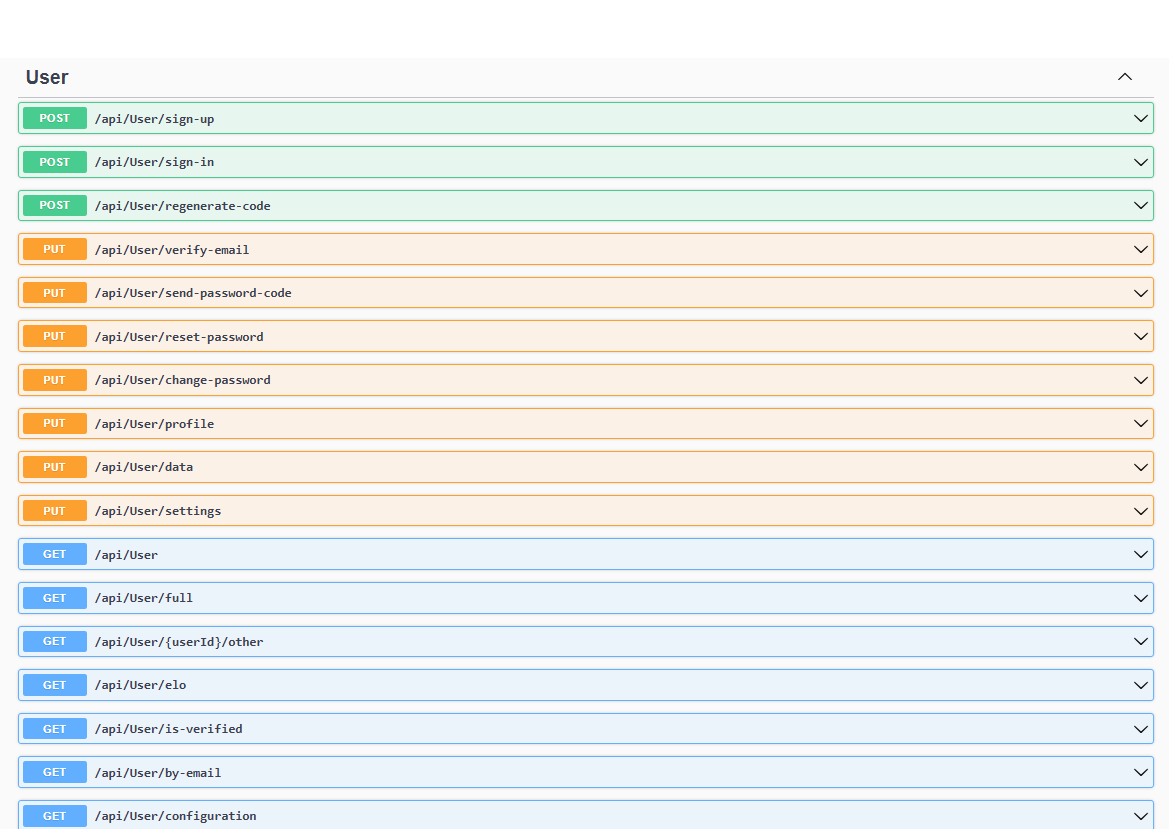
\includegraphics[width=1\textwidth]{zdj/user_controller.png}
        \caption{Punkty końcowe API do rejestracji użytkowników, uwierzytelniania i zarządzania profilami.}
        
    \end{figure}

\newpage

    \item \textbf{FriendshipController}
    \begin{itemize} 
        \item \textbf{POST /api/friendship/invite} - Tworzy zaproszenie do znajomości z oczekującym statusem. 
        \item \textbf{POST /api/friendship/block} - Tworzy zaproszenie do znajomości z odrzuconym statusem. 
        \item \textbf{PUT /api/friendship/{friendshipId}/respond} - Zmienia status oczekującej znajomości (akceptacja lub odrzucenie zaproszenia). 
        \item \textbf{GET /api/friendship/all-by-status} - Pobiera wszystkich użytkowników z określonym statusem relacji (np. znajomi, oczekujący). 
        \item \textbf{GET /api/friendship/all-non} - Pobiera wszystkich użytkowników, którzy nie są w relacji z użytkownikiem. 
        \item \textbf{GET /api/friendship/{friendshipId}/profile} - Pobiera profil znajomego na podstawie identyfikatora znajomości. 
        \item \textbf{GET /api/friendship/ranking} - Pobiera ranking użytkowników wśród znajomych na podstawie wybranego modelu. 
        \item \textbf{GET /api/friendship/{friendshipId}/games} - Pobiera listę gier rozegranych w ramach znajomości. 
        \item \textbf{DELETE /api/friendship/{friendshipId}} - Usuwa znajomość i/lub odblokowuje użytkownika. 
    \end{itemize}
    \begin{figure}[h!]
        \centering
        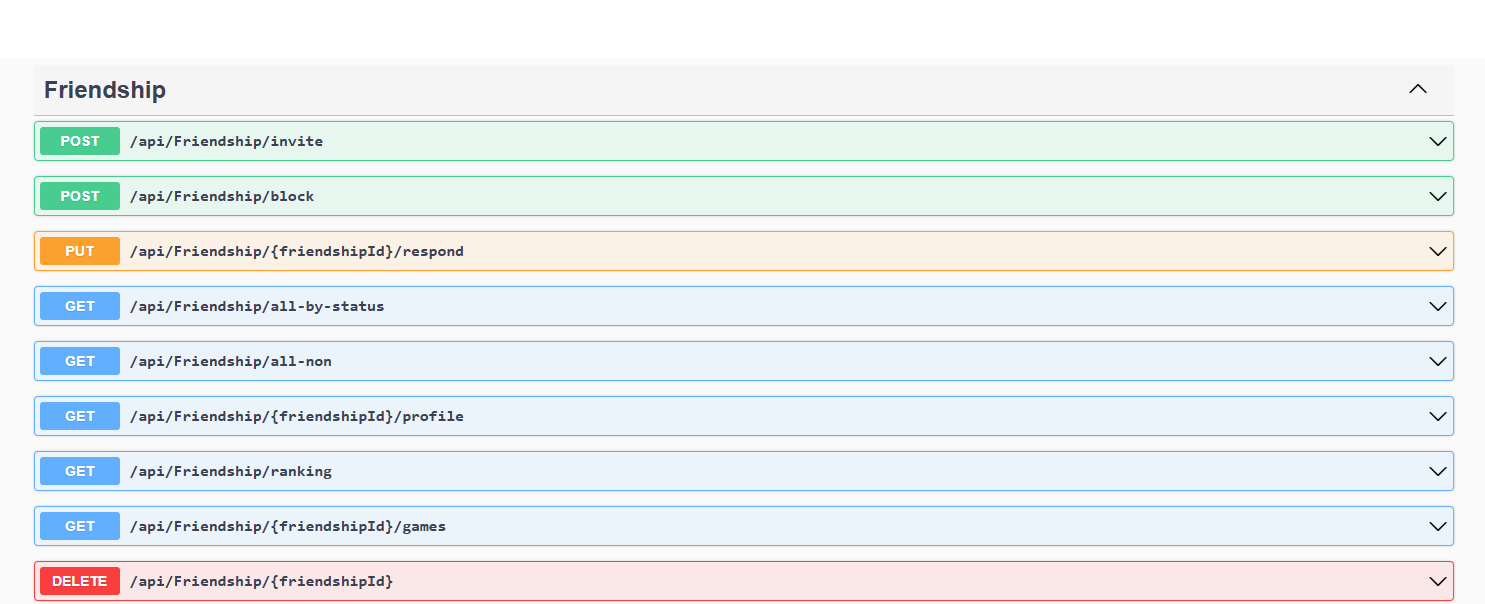
\includegraphics[width=1\textwidth]{zdj/friendship_controller.png}
        \caption{Punkty końcowe API do zarządzania zaproszeniami do znajomych, przyjaźniami i relacjami użytkowników.}
        
    \end{figure}

\newpage

    \item \textbf{WebGameController}
    \begin{itemize} 
        \item \textbf{POST /api/webgame/search} - Inicjuje poszukiwanie gry online, tworzy gracza i ustawia czas gry, jeśli nie istnieje. 
        \item \textbf{POST /api/webgame/private} - Tworzy prywatną grę i zwraca jej identyfikator. 
        \item \textbf{POST /api/webgame/email} - Tworzy prywatną grę przez podanie adresu e-mail przeciwnika, zwraca identyfikator gry. 
        \item \textbf{POST /api/webgame/link} - Tworzy prywatną grę z linkiem, który umożliwia dostęp do gry, zwraca identyfikator gry. 
        \item \textbf{GET /api/webgame/is-in-game} - Sprawdza, czy gracz jest już w grze. 
        \item \textbf{GET /api/webgame/{gameId}/update-required} - Sprawdza, czy wymagana jest aktualizacja stanu gry dla gry stworzonej za pomocą linku. 
        \item \textbf{GET /api/webgame/{gameId}} - Pobiera dane jednej gry na podstawie identyfikatora gry. 
        \item \textbf{GET /api/webgame/{gameId}/player} - Pobiera dane gracza w danej grze. 
        \item \textbf{GET /api/webgame/{gameId}/time} - Pobiera czas pozostały dla gracza w danej grze. 
        \item \textbf{GET /api/webgame/{gameId}/opponent} - Pobiera dane przeciwnika z zakończonej gry. 
        \item \textbf{GET /api/webgame/{gameId}/timing} - Pobiera konfigurację czasu gry (timing) dla danej gry. 
        \item \textbf{GET /api/webgame/all-ongoing} - Pobiera wszystkie aktywne gry dla użytkownika. 
        \item \textbf{GET /api/webgame/all-finished} - Pobiera wszystkie zakończone gry dla użytkownika. 
        \item \textbf{GET /api/webgame/type-history} - Pobiera historię gier dla wybranego typu czasu gry. 
        \item \textbf{GET /api/webgame/invitations} - Pobiera wszystkie zaproszenia do gier, które zostały jeszcze nieodebrane. 
        \item \textbf{GET /api/webgame/{gameId}/messages} - Pobiera wszystkie wiadomości z danej gry. 
        \item \textbf{GET /api/webgame/stats} - Pobiera statystyki wszystkich gier rozegranych przez użytkownika. 
        \item \textbf{DELETE /api/webgame/abort} - Anuluje poszukiwanie gry online. 
        \item \textbf{DELETE /api/webgame/{gameId}/cancel} - Anuluje prywatną grę, usuwając graczy. 
    \end{itemize}
    \begin{figure}[h!]
        \centering
        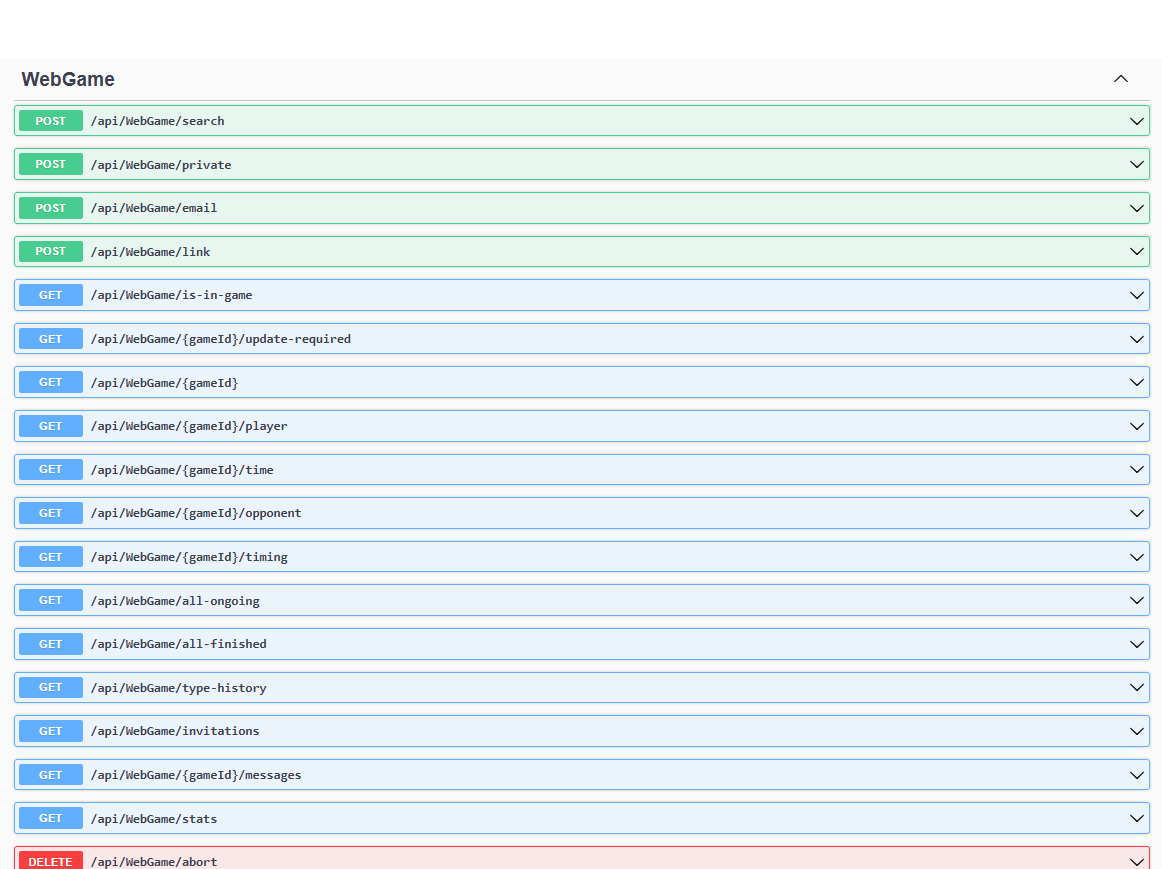
\includegraphics[width=1\textwidth]{zdj/webgame_controller.png}
        \caption{Punkty końcowe API do zarządzania grami sieciowymi, w tym wyszukiwania, tworzenia i sprawdzania statusu graczy w grach publicznych i prywatnych.}
        
    \end{figure}

\newpage

    \item \textbf{EngineGameController}
    \begin{itemize} 
        \item \textbf{POST /api/enginegame/start} - Rozpoczyna nową grę z silnikiem szachowym. 
        \item \textbf{POST /api/enginegame/{gameId}/make-move} - Wykonuje ruch w grze, wykonany przez gracza lub silnik.
        \item \textbf{PUT /api/enginegame/{gameId}/end-game} - Kończy grę z silnikiem szachowym. 
        \item \textbf{PUT /api/enginegame/{gameId}/change-engine} - Zmienia poziom trudności silnika szachowego. 
        \item \textbf{PUT /api/enginegame/{gameId}/undo-move} - Cofnięcie ostatniego wykonanego ruchu. 
        \item \textbf{PUT /api/enginegame/update-settings} - Aktualizuje ustawienia związane z grami z silnikiem szachowym. 
        \item \textbf{GET /api/enginegame/{gameId}} - Pobiera wszystkie dane dotyczące gry z silnikiem szachowym.
        \item \textbf{GET /api/enginegame/{gameId}/winner} - Pobiera zwycięzcę gry z silnikiem szachowym. 
        \item \textbf{GET /api/enginegame/{gameId}/engine-move} - Pobiera ruch wykonany przez silnik w grze. 
        \item \textbf{GET /api/enginegame/{gameId}/all-messages} - Pobiera wszystkie wiadomości związane z aktualną grą z silnikiem. 
        \item \textbf{GET /api/enginegame/all-games} - Pobiera wszystkie gry z silnikiem szachowym. 
    \end{itemize}
    \begin{figure}[h!]
        \centering
        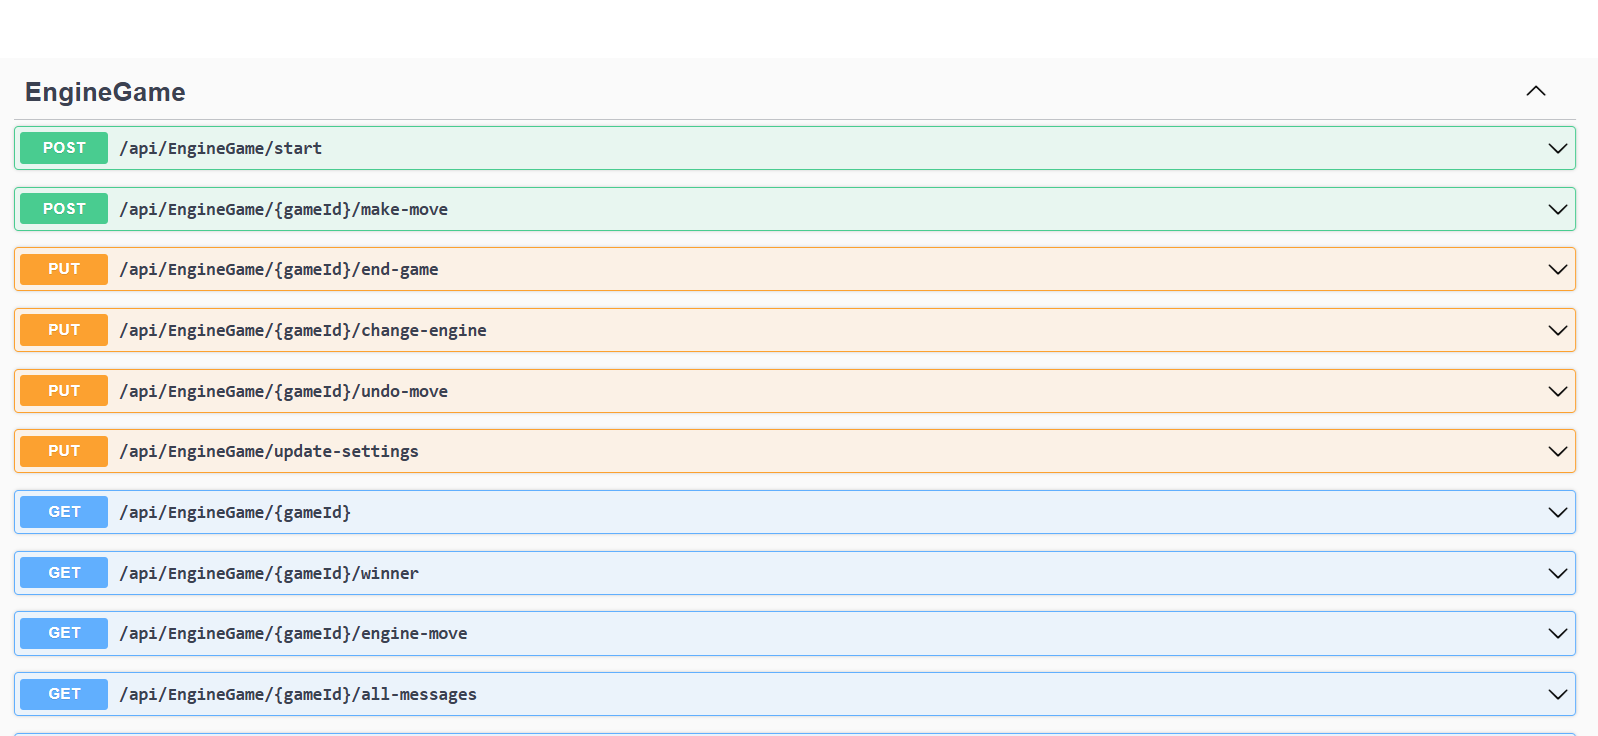
\includegraphics[width=1\textwidth]{zdj/enginegame_controller.png}
        \caption{Punkty końcowe API do zarządzania grami silnika, w tym uruchamiania, wykonywania ruchów, zmiany ustawień i przeglądania danych gry.}
        
    \end{figure}
\end{itemize}

\newpage

        \subsubsection{Entity Framework Core}


    \subsection{Frontend}
        \subsubsection{Architektura}
Modułowa architektura frontendu
\\\\
Termin ten kładzie nacisk na podział aplikacji na modułowe części wielokrotnego użytku, takie jak "components", "pages", "hooks" i "services". Każdy moduł ma jasny cel, co ułatwia zarządzanie i skalowanie.


\subsubsection{Wykorzystane biblioteki}

\begin{itemize}
    \item \textbf{@microsoft/signalr}: Biblioteka SignalR od Microsoftu pozwala na komunikację w czasie rzeczywistym między aplikacjami frontendowymi a serwerem. Jest to kluczowa biblioteka, umożliwiająca implementację funkcji czatu lub powiadomień w czasie rzeczywistym, np. w grze szachowej, w której użytkownicy mogą odbierać i wysyłać wiadomości na żywo.
    \item \textbf{@mui/x-charts}: Biblioteka wykorzystywana do tworzenia interaktywnych wykresów i wizualizacji danych w aplikacjach React. Może być używana do wyświetlania analiz, statystyk lub wyników gier w postaci wykresów.
    \item \textbf{@types/jsonwebtoken}: Typy TypeScript dla biblioteki jsonwebtoken. Używane do pracy z tokenami JWT (JSON Web Tokens), które mogą być wykorzystywane do uwierzytelniania i autoryzacji użytkowników w aplikacjach webowych.
    \item \textbf{axios}: Klient HTTP, który ułatwia wykonywanie zapytań do API. Jest to popularne narzędzie do pracy z zapytaniami typu GET, POST, PUT, DELETE i innymi, pozwalające na łatwą obsługę odpowiedzi z serwera, w tym błędów.
    \item \textbf{guid-typescript}: Biblioteka umożliwiająca generowanie i operowanie na identyfikatorach GUID (Globally Unique Identifiers) w aplikacjach TypeScript. Może być używana do generowania unikalnych identyfikatorów, np. dla nowych gier, użytkowników lub sesji.
    \item \textbf{history}: Biblioteka zarządzająca historią przeglądarki, używana przez react-router-dom do zarządzania nawigacją w aplikacjach SPA (Single Page Application). Pozwala na manipulowanie historią przeglądarki (np. przechodzenie do nowych stron bez przeładowania strony).
    \item \textbf{jsonwebtoken}: Biblioteka do tworzenia i weryfikacji tokenów JWT. JWT jest szeroko stosowanym standardem w aplikacjach webowych do zarządzania uwierzytelnianiem i autoryzacją użytkowników.
    \item \textbf{jwt-decode}: Biblioteka do dekodowania tokenów JWT. Pomaga w ekstrakcji informacji z tokenów, takich jak dane użytkownika lub czas wygaśnięcia tokenu.
    \item \textbf{msw}: Mock Service Worker – biblioteka służąca do tworzenia fikcyjnych serwisów (mocking API). Używana do testowania aplikacji frontendowych bez konieczności posiadania aktywnego backendu. Może służyć do mockowania odpowiedzi z API w trakcie rozwoju lub testów.
    \item \textbf{react}: Podstawowa biblioteka do budowy interfejsów użytkownika w aplikacjach frontendowych. React jest wykorzystywany do tworzenia dynamicznych komponentów UI, które mogą się aktualizować w odpowiedzi na zmiany w danych.
    \item \textbf{react-dom}: Zawiera funkcje do renderowania aplikacji React na stronie HTML. Jest to kluczowy komponent w ekosystemie React, umożliwiający integrację z DOM.
    \item \textbf{react-router-dom}: Biblioteka do obsługi routingu w aplikacjach React. Umożliwia tworzenie linków, trasowanie i zarządzanie nawigacją między różnymi widokami (stronami) w aplikacji SPA.
    \item \textbf{sass}: Preprocesor CSS, który pozwala na pisanie bardziej zorganizowanego i modularnego CSS. Zawiera funkcje takie jak zmienne, zagnieżdżanie, mixiny, które ułatwiają pisanie i utrzymanie kodu stylów.
    \item \textbf{scss}: Skrócona nazwa dla SASS (Syntactically Awesome Stylesheets). SCSS to rozszerzenie składni SASS, które jest bardziej zbliżone do standardowego CSS i jest szeroko stosowane w nowoczesnych aplikacjach frontendowych.
    \item \textbf{uuid}: Biblioteka do generowania unikalnych identyfikatorów UUID. Jest często używana w aplikacjach do generowania identyfikatorów dla elementów lub sesji.
    \item \textbf{@eslint/js}: Biblioteka ESLint dla JavaScript, wykorzystywana do sprawdzania jakości kodu, wychwytywania błędów i utrzymywania spójnego stylu kodowania w zespole.
    \item \textbf{@testing-library/dom}: Biblioteka do testowania DOM w aplikacjach frontendowych, pozwala na tworzenie testów jednostkowych i integracyjnych w React.
    \item \textbf{@testing-library/react}: Biblioteka wspomagająca testowanie komponentów React, która integruje się z popularnymi narzędziami do testów, takimi jak Jest i React Testing Library.
    \item \textbf{eslint}: Narzędzie do statycznej analizy kodu, wykorzystywane do zapewnienia jakości i spójności kodu JavaScript/TypeScript, zgodnie z określonymi zasadami.
    \item \textbf{stylelint}: Narzędzie do analizy CSS i SCSS, które pomaga w utrzymaniu porządku i jakości kodu stylów.
    \item \textbf{typescript}: Typowanie statyczne dla JavaScriptu. TypeScript dodaje do JavaScript typy i inne funkcje, które pomagają uniknąć błędów w kodzie i poprawiają skalowalność aplikacji.
    \item \textbf{vite}: Szybki bundler i serwer deweloperski, który wspiera nowoczesne technologie, takie jak ES Modules, TypeScript i React, zapewniając szybki czas ładowania podczas pracy nad projektem.
    \item \textbf{vitest}: Framework do testowania w ekosystemie Vite. Umożliwia szybkie uruchamianie testów jednostkowych, które są zgodne z biblioteką Jest, ale zoptymalizowane pod kątem Vite.
\end{itemize}

\newpage
\section{Instrukcja obsługi}

\newpage

\section{Testy}
    \subsection{Frontend}
        \subsubsection{Testy automatyczne}
        \subsubsection{Testy maunalne}
    \subsection{Backend}
        \subsubsection{Testy jednostkowe}
Test jednostkowy to kod wykonujący inny kod w kontrolowanych warunkach w ramach jednego procesu w pamięci, w celu weryfikacji (bez ingerencji programisty), że testowana logika działa w ściśle określony sposób.
\\\\
W niniejszym projekcie testy jednostkowe zostały wykorzystane w celu automatycznej kontroli poprawności działania klas obsługującym otrzymane zapytania (RequestHandler). Do każdego przypadku obsługi został utworzony test, sprawdzający zarówno poprawną realizację procedury oraz kazdy z możliwych i zaimplementowanych opcji niepoprawnego zapytania.
\\\\


        \subsubsection{Testy integracyjne}
Testy integracyjne to etap w procesie tworzenia oprogramowania, który polega na łączeniu i sprawdzaniu, jak ze sobą współpracują różne części systemu. Mają na celu identyfikację potencjalnych błędów i niezgodności, które mogą pojawić się podczas interakcji między różnymi modułami. Zaczynając, należy pamiętać, że osiągniecie powodzenia w testach integracyjnych wymaga zrozumienia całej struktury systemu, jak również umiejętności identyfikacji kluczowych punktów interakcji. Jest to proces wymagający, ale dający wartościowe informacje powiązane z ogólnym działaniem aplikacji.



\newpage
\section{Podsumowanie}

\newpage
\section{Literatura}

\begin{itemize}
    \item https://react.dev/learn/describing-the-ui
    \item https://vitejs.dev/guide/
    \item https://en.wikipedia.org/wiki/Chess
    \item https://boringowl.io/blog/testy-integracyjne-plusy-i-minusy-ich-stosowania
    \item https://devstyle.pl/2020/06/25/mega-pigula-wiedzy-o-testach-jednostkowych/
    \item https://boringowl.io/tag/figma
    \item https://justjoin.it/blog/wszystko-co-musicie-wiedziec-o-javascript-co-to-dla-kogo-i-ile-zarobimy
    \item https://www.droptica.pl/blog/co-jest-typescript-i-dlaczego-sprawdzi-sie-w-twoich-projektach/
    \item https://boringowl.io/blog/przeglad-vitejs-nowa-generacja-narzedzi-do-budowania-aplikacji-front-end
    \item https://boringowl.io/blog/poznaj-sass-zyskaj-kontrole-nad-stylem-swojej-strony
    \item https://blog.strefakursow.pl/jezyk-c-czym-jest-i-gdzie-sie-go-uzywa/
    \item https://learn.microsoft.com/pl-pl/dotnet/framework/get-started/
    \item https://www.ovhcloud.com/pl/learn/what-is-postgresql/
    \item https://learn.microsoft.com/pl-pl/devops/develop/git/what-is-git
    \item https://coderslab.pl/pl/blog/github-co-to-jest-i-do-czego-sluzy
    \item https://polontech.com/pl/sourcetree/
    \item https://www.droptica.pl/blog/co-jest-postman-do-czego-sluzy-i-jakie-sa-jego-funkcjonalnosci/
    \item https://www.ovhcloud.com/pl/learn/what-is-rest-api/
\end{itemize}

\end{document}
